\documentclass{article}
\usepackage{graphicx}
\usepackage{mathtools}
\usepackage{amssymb}
\usepackage[backend=bibtex]{biblatex}
\addbibresource{Proposal.bib}
\usepackage[margin=.5in]{geometry}
\usepackage{setspace}
\linespread{1.5}
\begin{document}

\section{Research Aims for PhD Candidacy}

Nicotinic acetylcholine receptors (nAChRs) are excitatory pentameric ligand gated ion channels (pLGICs) found through out the central and peripheral nervous system. Function of these neurotransmitter receptors is very sensitive to composition of the surrounding lipid membrane. However, the mechanisms of interaction between nAChR and its lipid environment are poorly understood. Research has shown a requirement for cholesterol in reconstitution mixtures of nAChR and other neuronal pLGICs, but other potentially essential lipids abundant in native membranes (particularly n−3 polyunsaturated fatty acids or PUFAs) have not been investigated.

\textit{Xenopus} oocytes have been used by experimentalists to test nAChR functionality with varying degrees of success. These oocytes have dramatically different membrane compositions ,when compared to native nAChR membranes, particularly in the location of unsaturation sites in long-tailed PUFAs. Translocation of neuronal membranes into oocytes has been shown to improve function of other lipid-sensitive pLGICs such as with $\gamma$-Aminobutyric acid (GABAa) receptors, but simpler supplementation of specific lipids has not, to our knowledge, been attempted. We propose a series of coarse grained simulations analyzing nAChR’s boundary lipids and partitioning behaviors, as well as associated tools to characterize elastic properties. This research will have implications for experimentalists using model cell lines to study function of pLGICs, as well as researchers looking to understand and treat disorders involving pLGIC signaling with associated lipid changes, and computational biochemistry and biophysics interested in membrane elasticity. I propose three aims for my PhD proposal:

\begin{enumerate}
  \item \textbf{Coarse-grained simulations of multiple subtypes of mammalian pLGICs in quasi-physiological membranes}  We observe nAChR partitioning into n-3 (DHA) rich domains with DHA-PE as nAChR’s primary boundary lipid. \textit{Xenopus} oocytes lipid composition are considerably different from neuronal membranes, but due to the observed affinity of DHA chains for nAChR , we believe adding small concentrations of n-3 is likely to restore the native boundary lipids. We will model various n-3 supplemented quasi-physiological membranes (such as oocytes) to predict those likely to provide a native local environment within an oocyte, for later testing by an experimental collaborator (Dr. John Baenziger of University of Ottawa). %We observe nAChR partitioning into n-3 (DHA) rich domains with DHA-PE as nAChR’s primary boundary lipid. Xenopus oocytes lipid composition are considerably different from neuronal membranes, but due to the high affinity of DHA chains for nAChR , a modest supplementation scheme is likely to restore the native boundary lipids. We will model various supplementation schemes to predict those likely to provide a native local environment within an oocyte, for later testing by an experimental collaborator (Dr. John Baenziger of University of Ottawa).

  \item \textbf{Investigation of the relative importance of pLGIC sequence versus shape in determining preferred lipid domain} This can be tested comparing effects on partitioning profiles upon mutation of lipid facing residues versus adjustments in membrane lipid composition. If the effect of the protein's sequence is measured to be greater than its shape, it is likely that pLGICs will display significant variation in partitioning behavior and annular lipid preferences. If the reverse is observed, it is likely that overall pLGIC shape and relative flexibility of domains drives partitioning; which may be shared across all pLGIC. %This can be tested comparing effects on partitioning profiles upon mutation of lipid facing residues versus adjustments in membrane lipid composition. If the former has a stronger effect, it is likely that pLGICs will display significant variation in partitioning behavior and annular lipid preferences, while if the latter has a stronger effect, it is likely that overall pLGIC shape and relative flexibility of domains drives partitioning, with similar preferences across the pLGIC family.

  \item \textbf{Development and release of a user-friendly VMD plugin for measuring elastic parameters of heterogenous membranes} This package could be of significant use to both chemists and biophysicists. It would allow computational researchers to easily predict the elasticity moduli of a membrane composed of a general lipid mixture. Combined with VMD’s convenient scripting environment, this alleviates the daunting nature of solving for the fluctuation spectrum and related moduli. While multiple individuals have developed scripts to determine the fluctuation spectrum of membranes, there is no universal tool computational chemists and biophysicists can use. This tool will assist us in optimizing lipid selections for modeled neuronal membranes; we can adjust lipid species and lipid concentrations to mimic elastic properties of neuronal membranes. 
\end{enumerate}

\newpage

\section{Significance of Proposed Research}
The nicotinic acetylcholine receptor (nAChR) is an excitatory pentameric ligand gated ion channel (pLGICs, previously known as “Cys-loop” receptors) found throughout the central and peripheral nervous system. It is critical for synaptic neurotransmission, is a target for various agonists including nicotine and general anesthetics \cite{Bondarenko_NMR_2013,Jayakar_Identification_2013,Ryan_Structural_1996,Mantipragada_Lipid_2003} and is implicated in addiction, schizophrenia, Alzheimer’s disease, spinal muscular atrophy, and neurological autoimmune disease \cite{MartinRuiz_4_1999, Arnold_Reduced_2004,Lennon_Immunization_2003,Papke_The_2012,Picciotto_Neuroprotection_2008}.  Although nAChRs are not exclusively found in post-synaptic membranes, they can be found at densities up to $10^4$$\mu m^2$ in post-synaptic membranes and their role in such membranes is most widely studied \cite{Bermdez_Partition_2010,Zuber_Structure_2013}.

Post-synaptic membranes in particular have distinctive lipid compositions, with elevated levels of n-3 PUFAs, cholesterol, and the phospholipid head group phosphoethanolamine (PE), and low abundance of monounsaturated acyl chains and sphingomyelin. \cite{Breckenridge_Adult_1973,Cotman_Lipid_1969}; this composition is closer to the electric organs of electrogenic fish \cite{Bara89,Quesada_Uncovering_2016} than to typical mammalian cell membranes.

Deviations from neuronal lipid concentration can occur due to aging and health related disorders, including disorders for which nAChRs are also implicated. Supplementing medication for schizophrenia with the n-3 PUFA eicosapentaenoic acid (EPA) has shown to improve schizophrenia symptoms in some patient populations \cite{Peet2003,Freemantle2006,Su2003} while a role for nicotine in reducing symptoms of schizophrenia is well established \cite{Picciotto2008}. Imbalance in membrane lipids may lead to a number of health issues such as diabetes and Alzheimer’s disease, and may alter pathway signaling leading to lipidosis \cite{Escriba2017,Laforet2010,Yadav2014}.

\section{Aim 1: Coarse-grained simulations of multiple subtypes of mammalian pLGICs in quasi-physiological membranes}
\begin{figure}[t!]\center
	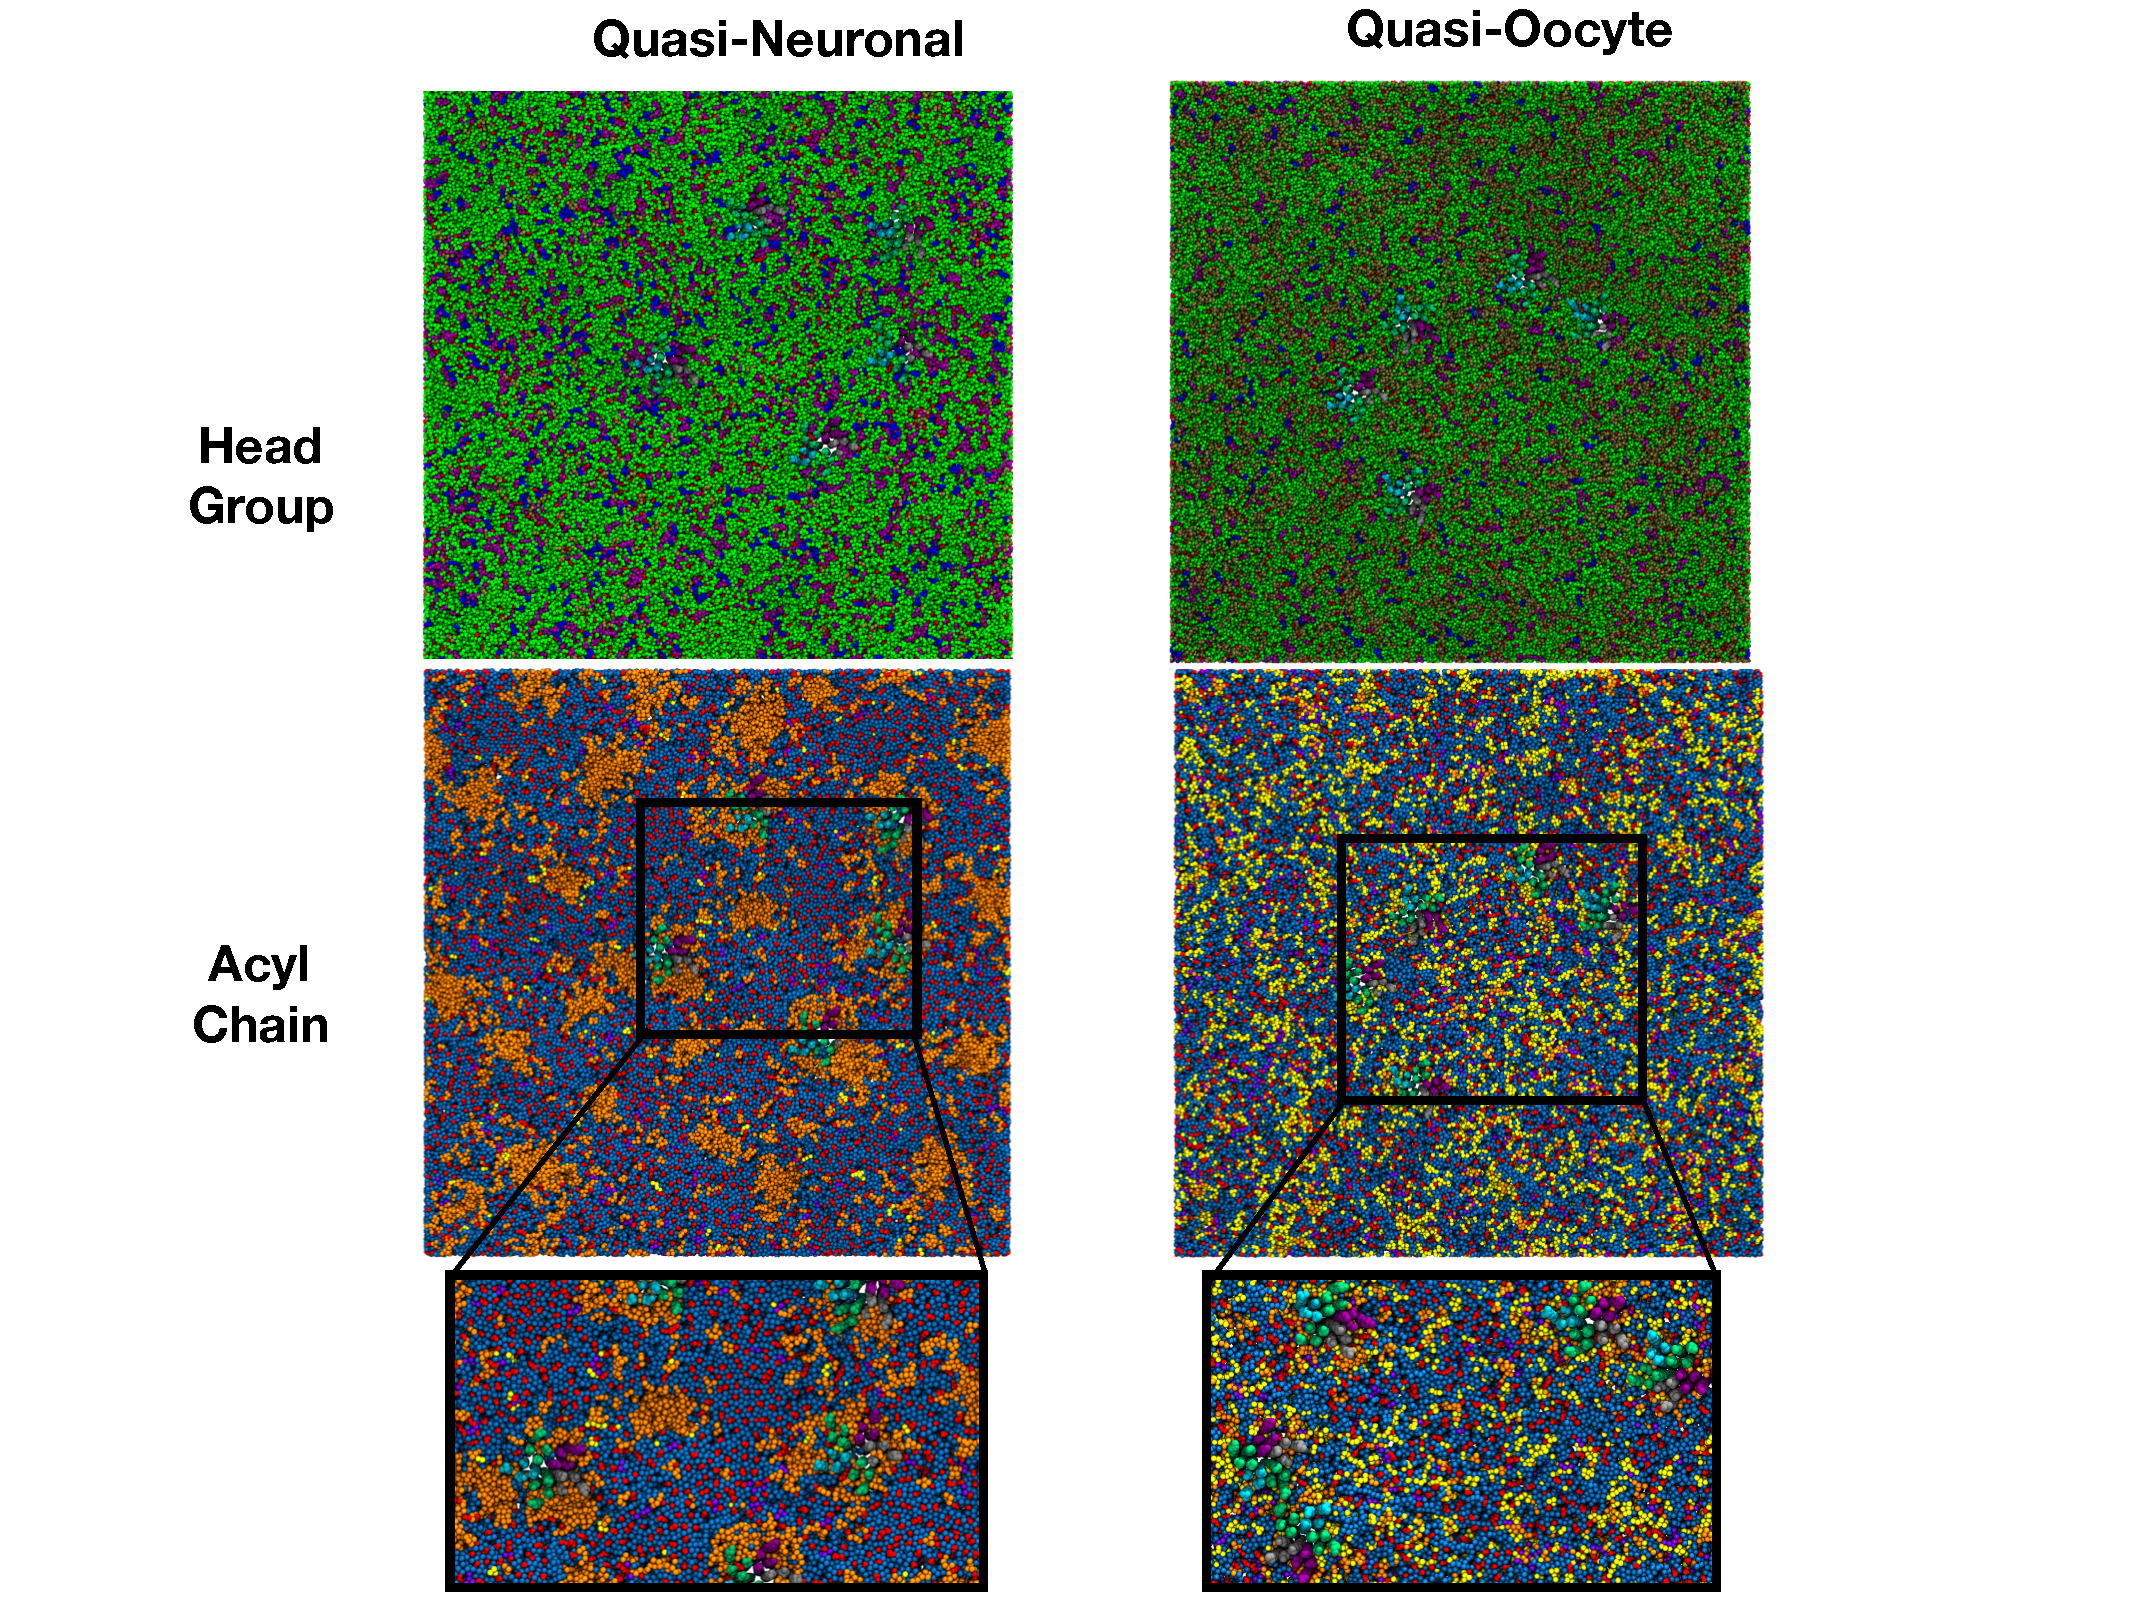
\includegraphics[width=11cm]{./F31/Memb_Comp.pdf}
	\caption{Comparison of nAChR lipid sorting in quasi-Neuronal and quasi-Xenopus oocyte membranes, according to either phospholipid head-group or location of acyl chain unsaturation, from coarse-grained MD simulations. nAChR transmembrane domain is shown in surface representation, colored by subunit. Top row: PE (purple), PC (green), SM (tan), PS (blue), cholesterol (red). Bottom Row: n-3 (orange), n-6 (yellow), n-9 (purple), saturated (blue), cholesterol (red). Composition of quasi-Neuronal and quasi-Oocyte membranes reflects all species that are sufficiently abundant to yield at least 2 molecules in a membrane of the simulated size.}
	\label{fig:ooct}
\end{figure}

pLGICs have complex gating behavior and structural requirements, and nAChRs are some of the most complex pLGICs. One of the most poorly understood components of nAChR is its unpredictable functional sensitivity to slight changes in its lipid environment, a property shared to a lesser extent by other pLGICs \cite{M.CriadoH.Eibl1982,Conti2013}.

Considerable experimental effort \cite{Fong_Correlation_1986,Sunshine_Lipid_1992,Hamouda_Assessing_2006,Butler_FTIR_1993,Bhushan_Correlation_1993,Fong_Stabilization_1987,Corrie_Lipid_2002} was expended, primarily in the 1980s and 1990s, to understand the underlying mechanism of nAChR lipid sensitivity, including identifying the likelihood of specific boundary lipids. Experimental studies focused primarily on cholesterol, which were required in native membranes (20-40\% of lipid composition) to support native levels of ion flux in purified and reconstituted nAChR \cite{Fong_Correlation_1986,Fong_Stabilization_1987}. Further experiments showed that while cholesterol could be depleted from the bulk membrane, a second pool of cholesterol could not be removed from nAChR-containing membranes by depletion \cite{Leibel1987}. However, results were inconclusive regarding whether cholesterol was sufficient to restore nAChR function. Interestingly, soybean lipids (which are also high in n-3 PUFAs) \cite{Yoshida1986,Regost2003,Olsen2003} are more effective at restoring ion flux than cholesterol alone \cite{Morales2006}.

\begin{figure}[t!]\center
	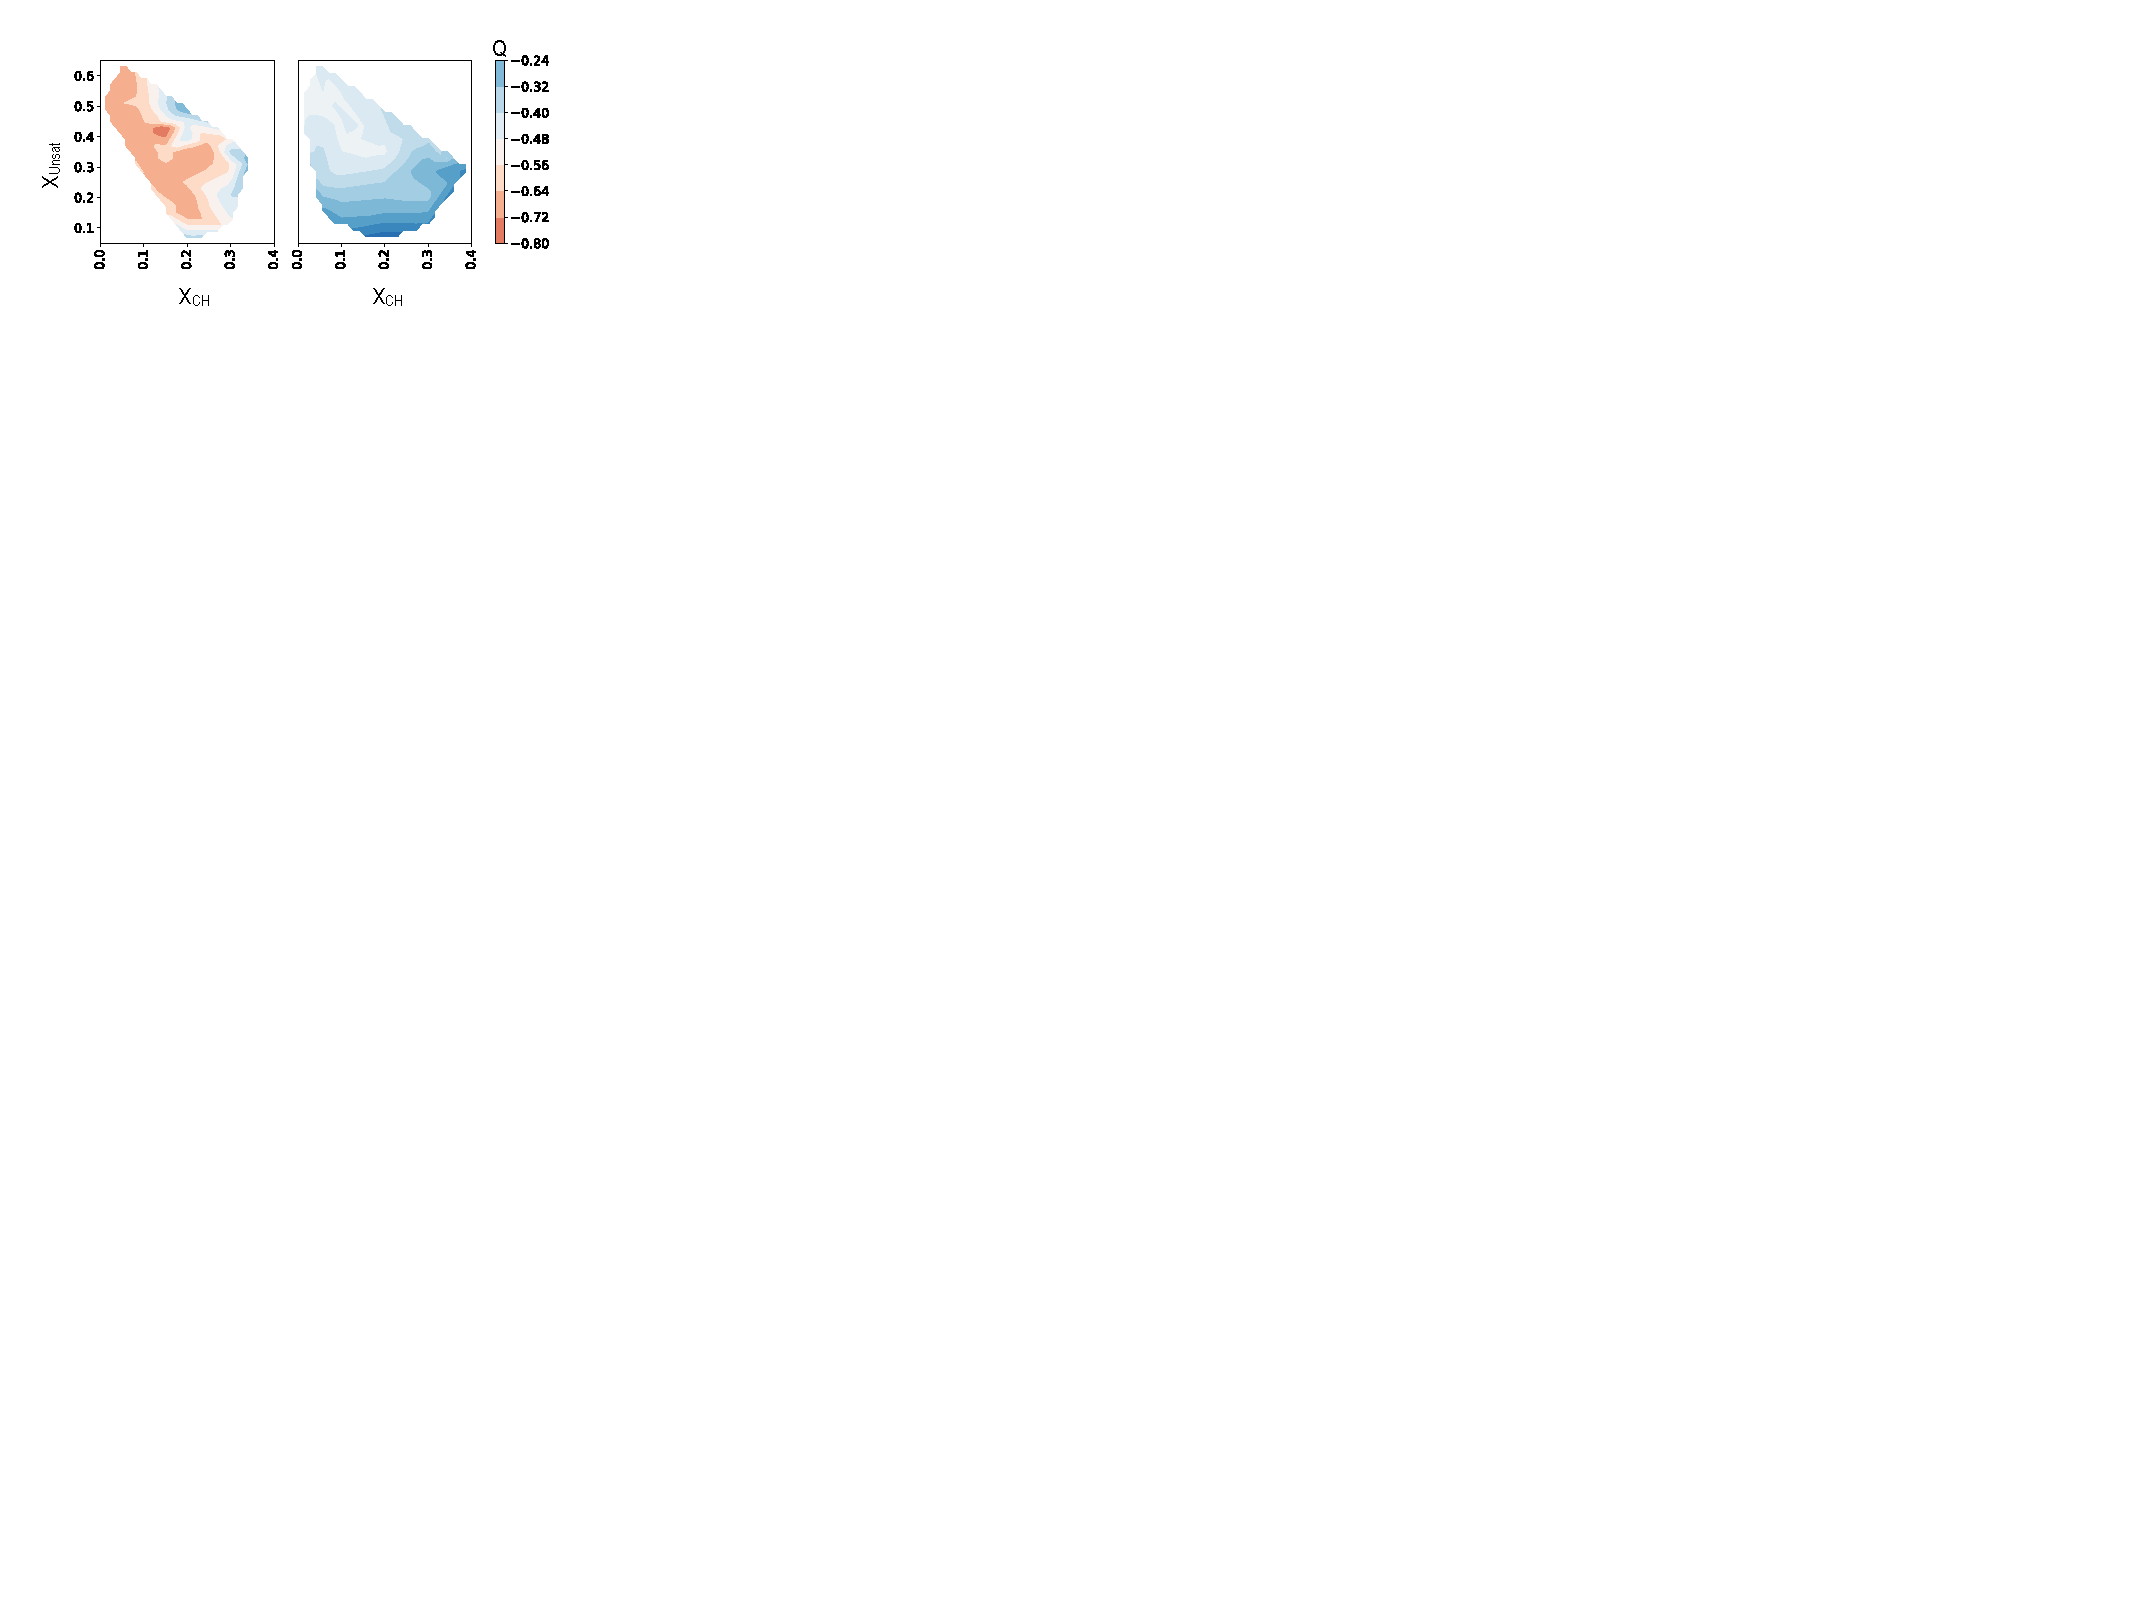
\includegraphics[width=11cm]{./F31/Q.pdf}
	\caption{Enrichment of nAChR annular lipids for saturated phospholipids in ternary mixture of cholesterol, saturated, and unsaturated phospholipids. $Q=\frac{\langle B_{SAT}\rangle_{ann}}{N_B\cdot x_{SAT}}-1$, where $\langle B_{SAT}\rangle_{ann}$ is the averaged fraction of boundary lipids composed of saturated phospholipids, $N_B$ is the total number of boundary lipids, and $x_{SAT}$ is the bulk mole fraction of saturated phospholipid chains. $Q>0$ indicates nAChR preference for the $l_o$ domain; $Q<0$ indicates nAChR preference for the $l_{do}$ domain.}
	\label{fig:Q}
\end{figure}

The working assumption in the time of most of those experiments was that the membrane was randomly mixed in the absence of protein, although lipid sorting by proteins was considered likely; there was little evidence available then that cholesterol by itself can induce non-random mixing and even domain formation in just a ternary lipid mixture. We are now also aware of the critical role of acyl chain unsaturation in this process, but previous experiments focused primarily on the role of cholesterol and phospholipid headgroup without including the lipids with n-3 PUFA chains that are so abundant in both the fish electric organ and the postsynaptic membrane.

It is still unknown what factors determine the lipids interacting directly with pLGICs , leading to a substantial source of uncertainty in present-day experiments and introducing a divergence between simulations and experiments that cannot be reasonably estimated. Ionic flux of reconstituted neuronal $\alpha$3$\beta$4nAChR expressed in Xenopus oocytes is less than 50\% of those expressed in mouse-fibroblasts, with neither consistently reproducing native behavior \cite{Fong_Correlation_1986,Sunshine_Lipid_1992,Hamouda_Assessing_2006,Butler_FTIR_1993,Bhushan_Correlation_1993,Fong_Stabilization_1987,Bednarczyk_Transmembrane_2002,Corrie_Lipid_2002}. Contrasts in membrane lipids may contribute significantly to these differences, and specific lipid incorporation may bypass the need for microtransplantation of entire sections of neuronal membranes \cite{Conti2013} into oocytes to achieve native function.
%It is still unknown what factors determine the lipids interacting directly with pLGICs , leading to a substantial source of uncertainty in present-day experiments and introducing a disparity between simulations and experiments that cannot be reasonably estimated. Conductance of recombinant neuronal a3b4nAChR expressed in Xenopus oocytes is less than 50\% of those expressed in mouse-fibroblasts, with neither consistently reproducing native behavior. [34] Differences in membrane lipids may contribute significantly to these differences, and rational lipid supplementation may forgo the need for microtransplantation of entire sections of neuronal membranes[35] into oocytes to achieve native function.

\subsection{Innovation of Research}

A large number of experiments, ranging from the straightforward to the particularly sophisticated, have been carried out to investigate the mechanisms underlying cholesterol modulation of pLGICs. The proposed studies involve investigation of lipid interactions with nAChR via coarse grained molecular dynamics. Numerous simulations of nAChR and other pLGICs with atomic resolution, powerful methods for investigating direct interactions of receptors with small molecules, are also reported in the literature. In the absence of realistic estimates for the protein-local lipid composition, most such simulations embed the receptor in a model membrane composed of DOPC or POPC, with occasional inclusion of cholesterol.

My preliminary studies, which use CG simulations capable of equilibrating a quasi-native membrane, indicate that nAChR has a surprisingly strong preference for n-3 PUFAs (Figures \ref{fig:ooct} and \ref{fig:Q}) as boundary lipids. Although these lipids are abundant in most native nAChR membranes, including the electric organ, they had not been included in experiments (except via an abundance in soybean lipids). This surprising observation, if true, offers possible explanations for limited success of many previous experiments.

It further suggests that regardless of the bulk membrane composition, nAChR functions natively in a homogeneous local environment of n-3 PUFAs. Our proposal for reproducing native boundary lipids within an oocyte relies on both this simplicity and the large difference in abundance of n-3 PUFAs between the oocyte and the neuron, which suggests there is a qualitative difference in lipid environment. Microtransplantation of neuronal cell membranes into oocytes \cite{Conti2013} has been carried out and shown to improve ion flux through nAChRs embedded in oocyte membranes, but I will run calculations to inform an approach which restricts supplementation to a few species of preferred boundary lipid, and would substantially improves experimental control. These predictions will be tested by a collaborator of Dr. Brannigan’s, Dr. John Baenziger at University of Ottawa.

\subsection{Approach of Research}

We propose a series of simulations characterizing the boundary lipids surrounding nAChR embedded within a modified oocyte membrane, with the aim of finding the modifications which will reproduce native boundary lipids. Our initial simulation results suggests nAChR partitions into $l_{do}$ with long chained PUFAs as boundary lipids (see Figure \ref{fig:ooct} and \ref{fig:Q}).

The proposed simulations will involve quasi-Oocyte lipid membranes and supplementing them with boundary lipids found in neuronal membranes. Our preliminary simulations indicate that n-3 lipids, particularly DHA, are highly enriched among boundary lipids (both annular and non-annular). We observe the annular ring of n-3 lipids to be surrounded by an outer ring of n-6 lipids, and an even more distant ring of n-9 lipids at the interface with the $l_o$ phase.

Differences in the local lipid environments surrounding pLGIC when expressed in common lines for cultured cells will be obtained by computational microscopy; embedding nAChRs in membranes approximating various cell lines including post-synaptic membranes, and \textit{Xenopus} oocytes \cite{Lindi2001,Gamba2005}. 
%Must be a better way to write this..
%Differences in the local  environment of the pLGIC when expressed in common lines for cultured cells will be obtained by computational microscopy of nAChRs in membranes approximating native membranes, including post-synaptic membranes, as well as common expression systems including Xenopus oocytes[57]. 

It is possible (especially if elastic effects are essential) that increasing the number of receptors or the system size will modify these distributions. Therefore, the first step of this aim is improving realism of the simulations of nAChR in the neuronal membrane, by increasing the number of receptors to around ten, enforcing realistic leaflet asymmetry, and incorporating the newer $\alpha$4$\beta$2 nAChR structure \cite{Morales-Perez_X_2016}. 

Assuming differences in boundary lipids are maintained, the expression system membrane will have its composition iteratively adjusted to mimic supplementation via liposomes, then allowed to re-equilibrate the local lipid concentration around the receptor.

Currently, I envision an initial analysis of these simulations by calculating membrane mixing, boundary lipid composition, and lipid-protein non-annular binding. Due to the variety of lipid species involved, calculations will be grouped into two sets: lipid head group (i.e. PC, PE, PS...), and acyl chain saturation (i.e. sat, n-1, n-2, n-3, n-6). Preliminary simulations show n-3 dominate the boundary lipids when lipids with n-3 acyl chains are increased by concentrations as low as $\sim$5\%. These initial simulations, quasi-ooctyes with DHA increased to 15$\%$, show DHA to make the dominant boundary lipid. Figure \ref{fig:ooct} shows two of these simulations, using five proteins in quasi-neuronal and quasi-oocyte membranes, and composition asymmetry (albeit mammalian concentration asymmetry). While I have focused on DHA, both n-3 PUFAs, Eicosapentaenoic acid (EPA) and $\alpha$-Linolenic acid (ALA), should also be considered for oocyte modulation.

Once a prediction has been developed for supplementation that would preserve boundary lipids, it will be shared with an experimental collaborator of Dr Brannigan’s, Dr. John Baenziger, to be tested for improved nAChR function. If differences in boundary lipids are not observed, an enrichment protocol will be predicted for shifting the membrane viscoelastic properties to that of the native system.

\section{Aim 2: Investigation of the relative importance of pLGIC sequence versus shape in determining preferred lipid domain}

Neuronal signaling relies heavily on transmembrane proteins such as ion channels and receptors, which are embedded in membranes with distinctive lipid compositions. The multitude of PUFA's within nAChR native membranes does not necessarily discount them; in fact they may be critical to functionality. Such lipid dependence offers the organism numerous possibilities for lipid based regulation \cite{Lennon2003}. Need real citation...

%Neuronal signaling relies heavily on transmembrane proteins such as ion channels and receptors, which are embedded in membranes with distinctive lipid compositions. The differences in lipid composition are not restricted to lipids found at low concentrations; mammalian neuronal membranes are rich in PUFAs, PE headgroups, and cholesterol.Such lipid dependence offers the organism numerous possibilities for lipid based regulation. [36]

Separation of cholesterol and saturated phospholipids from unsaturated phospholipids, into liquid-ordered $l_o$ (“raft”) and liquid-disordered $l_{do}$ domains respectively, is detected even in simple ternary lipid mixtures. Increasing both cholesterol concentration and acyl chain unsaturation, as in neuronal membranes, increases the propensity of the membrane to form sharply-defined domains relative to other mammalian membranes.

\begin{figure}[t!]
	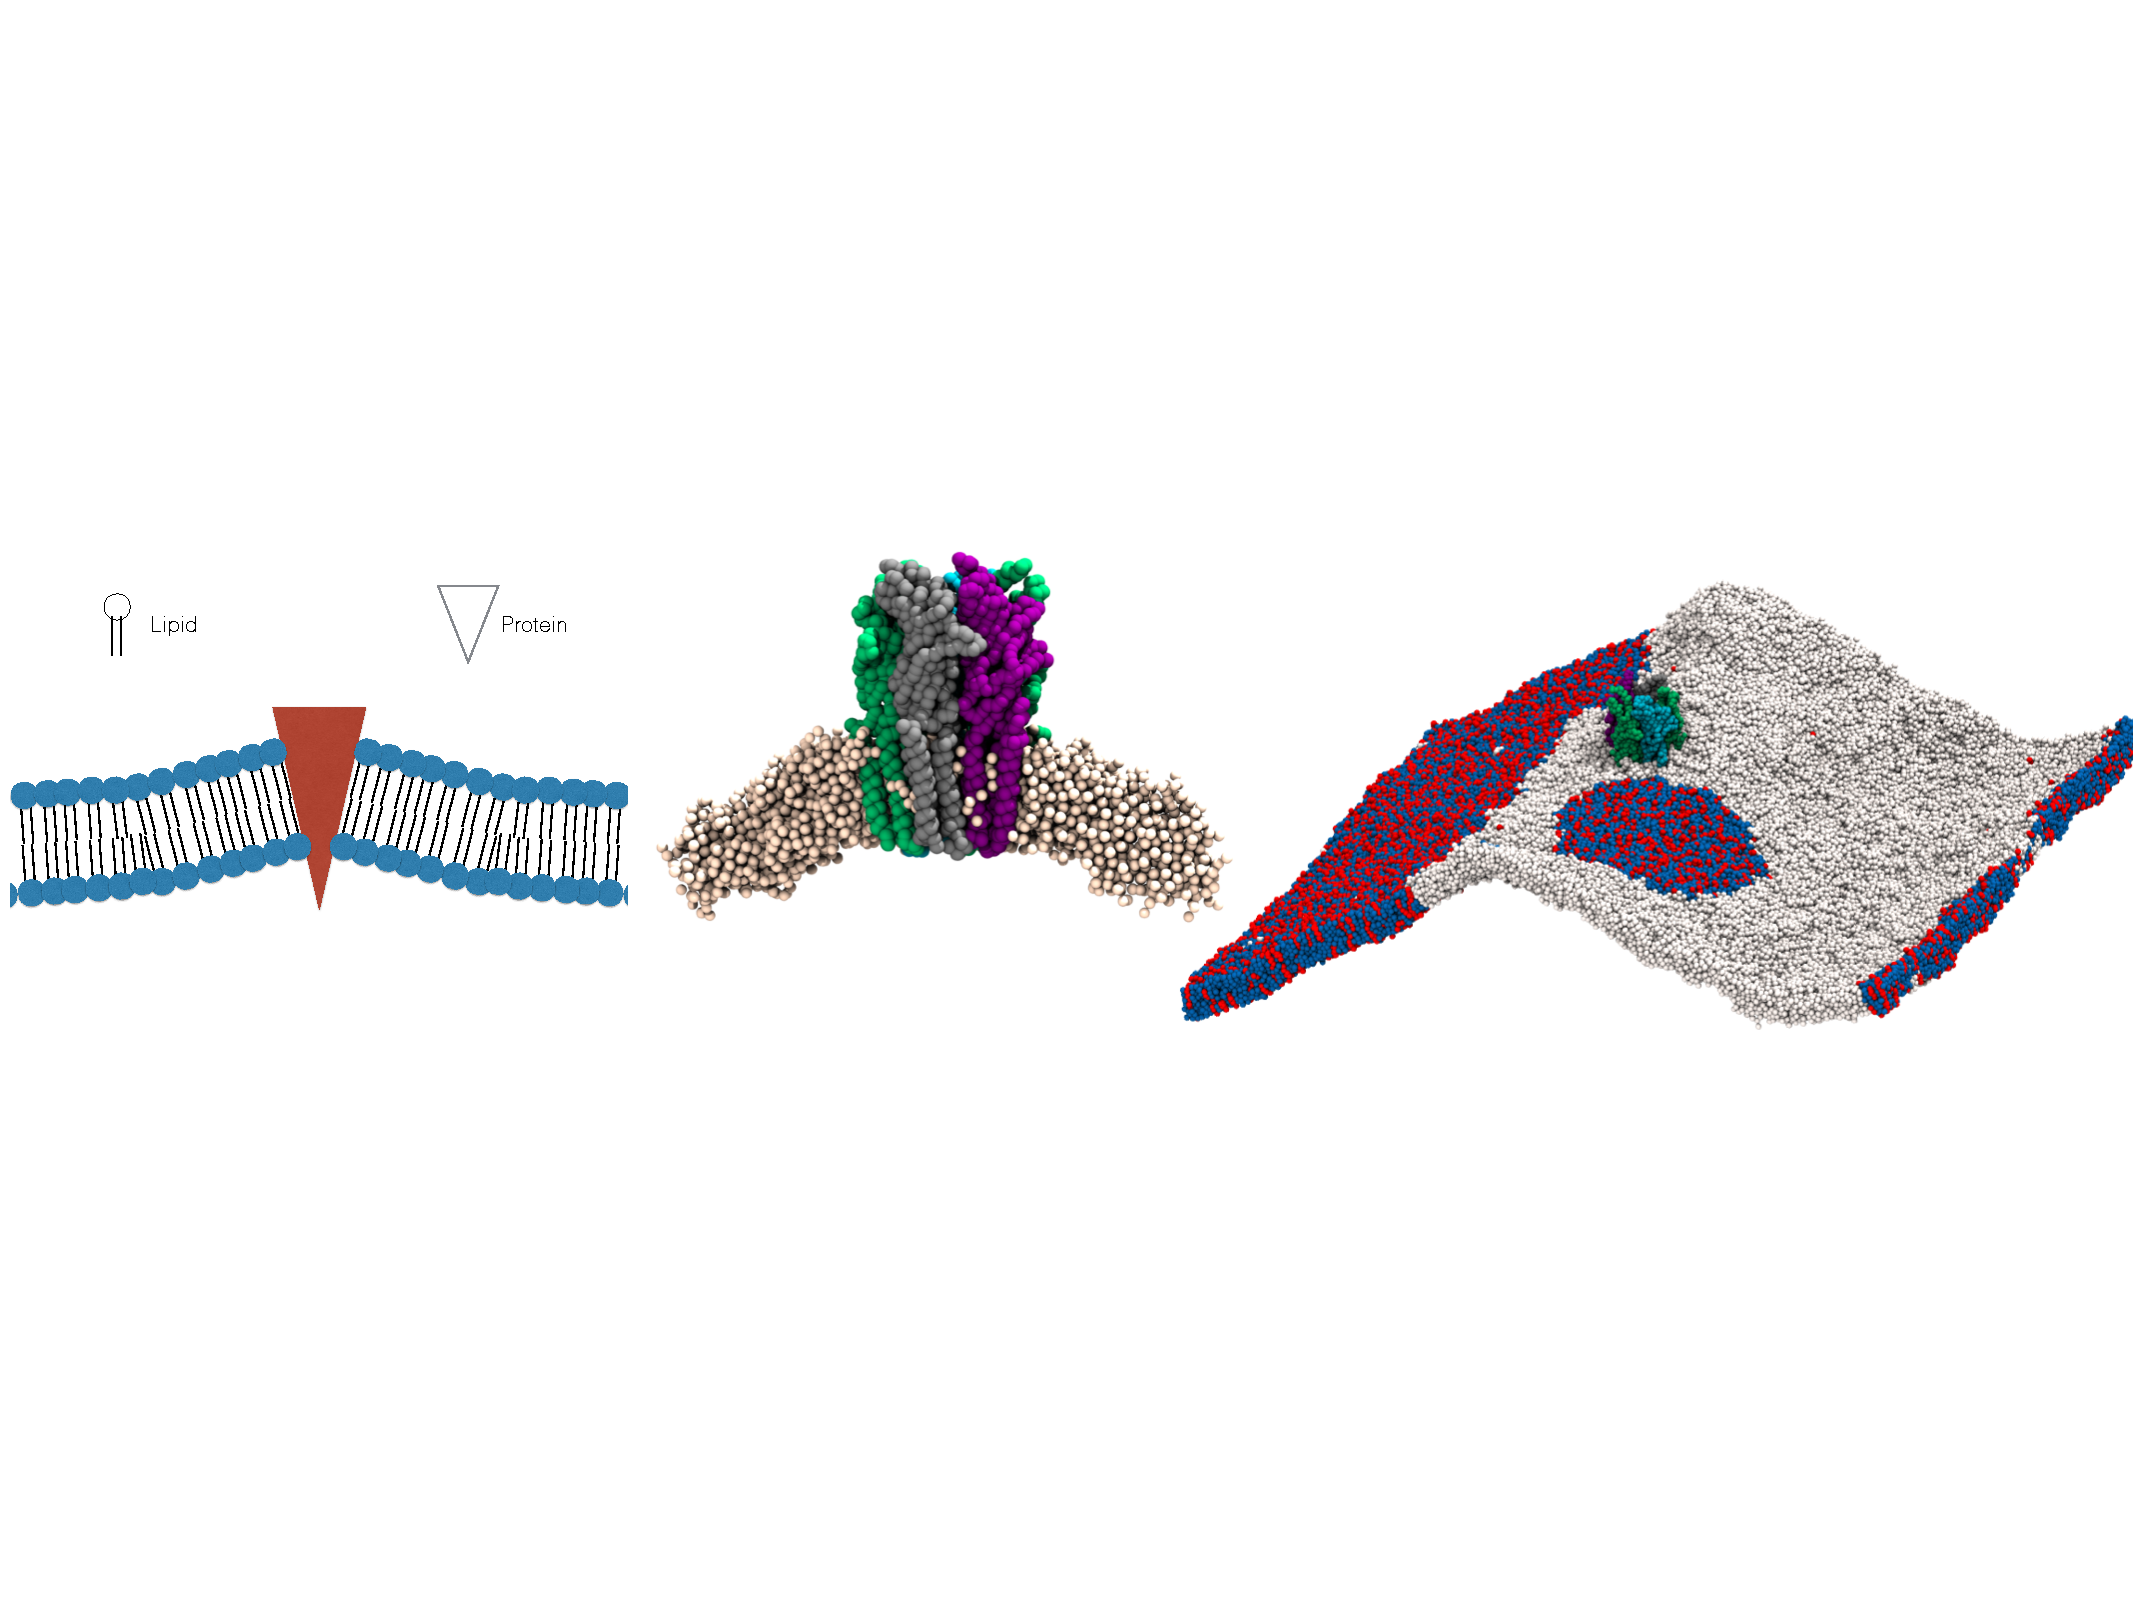
\includegraphics[width=20cm]{./F31/Curvature4.pdf}
	\caption{Possible role of membrane flexibility in determining nAChR partitioning. (A) A schematic representation of predicted membrane deformation around a cone-shaped protein, as described in Goulian et al, \cite{Goulian1996} in which the protein imposes constraints on the slope of the membrane at the interface with the protein (B) Cross-sectional cut of simulation-frame showing membrane deformation around nAChR embedded in an $l_{do}$ phase composed of DHA-PE (purple). (C) Phase-boundary partitioning in a larger membrane. nAChR is localized at the interface between the $l_{do}$ phase composed of DHA-PE and the $l_o$ phase composed of DPPC (green) and cholesterol (red). Provided the membrane is sufficiently large, partitioning at the boundary permits tangential interaction with the cholesterol-rich $l_o$ domain while the flexible $l_{do}$ domain still absorbs the energetic cost of deformation.}
	\label{fig:deform}
\end{figure}

\begin{figure}[t!]
	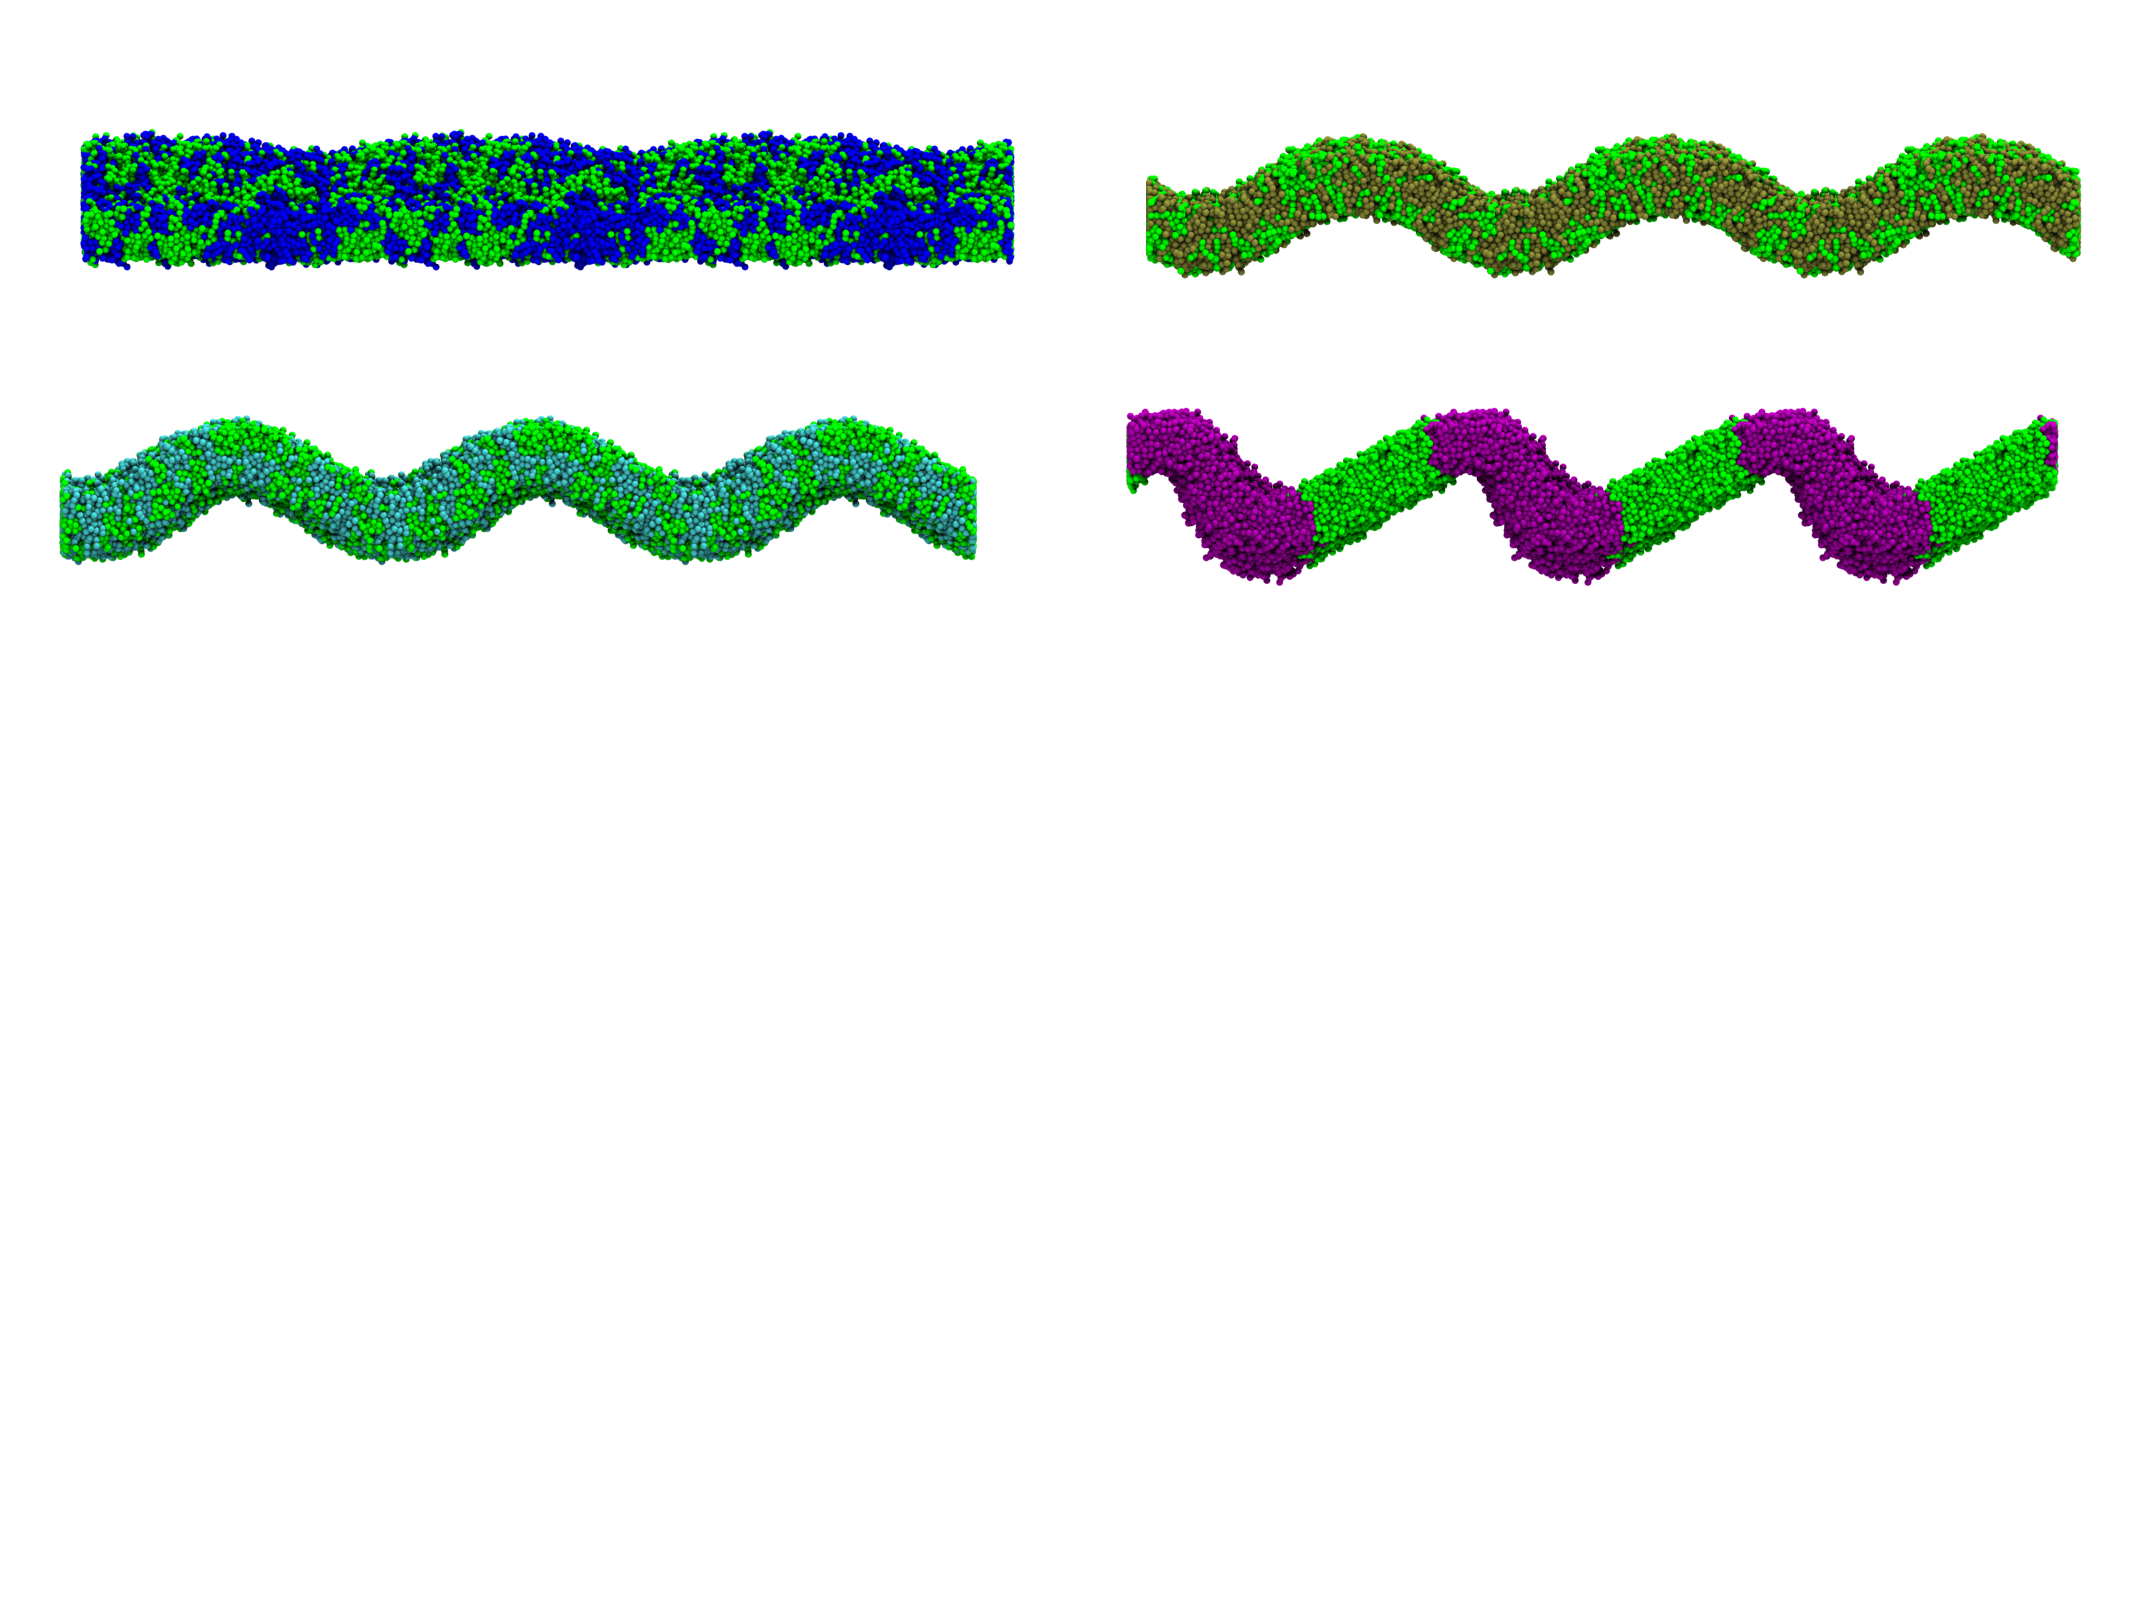
\includegraphics[width=20cm]{./F31/MultiImageElastic.pdf}
	\caption{ Binary, randomly-mixed membranes with increasing thermal undulations and decreasing bending modulus $k_c$. We predict that the more flexible membranes (lower $k_c$) will accommodate a cone shaped protein with reduced energetic costs. The bending modulus $k_c$ can be measured from the thermal undulation spectrum, as well as additional methods appropriate for small membranes. Aim 3 proposes implementation of these methods into a plugin for the widely used analysis-software VMD.}
	\label{fig:elast}
\end{figure}

As one example, neurotransmitter receptors must cluster at high density for efficient neurotransmission, and effects of lipid composition on membrane organization may serve an important modulatory role for an organism's ion channel functionality. The high density of nAChR clusters found in the postsynaptic membrane of the mature neuromuscular junction ($10^4$$\mu m^{-2}$) is well-established to be stabilized by dimerization of nAChRs via binding of the cytoplasmic peripheral membrane protein rapsyn \cite{Zuber_Structure_2013}. This process is also sensitive to membrane composition, particularly cholesterol. It has been frequently hypothesized \cite{Zhu2006,Bruses2001} that initial stages of clustering may require clustering via lipid domains, but experiments investigating whether nAChRs partition into lipid domains have been inconclusive \cite{Bermdez_Partition_2010,Perillo2016}.

Such experiments have focused primarily on detecting partitioning into liquid-ordered ($l_o$ ) domains, which is often detected differently than partitioning into $l_{do}$ domains; in my preliminary simulations we observe partitioning of nAChRs into the $l_{do}$ domain (Figure \ref{fig:ooct}). Partitioning into $l_{do}$ domains would also cluster receptors and be cholesterol dependent, but would be a less effective mechanism in low cholesterol membranes, such as oocytes.

\subsection{Innovation of Research}

Our observation that nAChR partitions into $l_{do}$ domains was surprising because these domains are very low in cholesterol; the simplest hypothesis to explain cholesterol-sensitivity of nAChR function and oligomerization was that nAChR would partition to the cholesterol rich $l_o$ “raft” phase, although experimental data has been inconclusive.

Direct visualization, using computational microscopy, of the $l_{do}$ domain around nAChR in the MD simulation trajectories revealed a deformation of the membrane around the cone-shape of the TMD (Figure \ref{fig:deform}). This type of deformation was predicted for a general cone shape protein two decades earlier, based on analytical elasticity theories of protein-induced membrane deformations \cite{Goulian1996,Weikl1998} but has not, to our knowledge, been used to predict partitioning preferences of proteins. According to these theories, the energetic penalty for the membrane deformation should increase with the bending rigidity $k_c$, so a significantly more flexible $l_{do}$ phase would be the natural preferred phase for a single receptor.

My approach for this aim is to better determine the role of membrane flexibility in pLGICs partitioning; this has not previously been considered in simulation or experimental design, but it will provide essential insight into whether domain preferences are likely to be more sensitive to pLGIC sequence or to differences in domain rigidity.

\subsection{Approach of Research}

If partitioning of pLGICs within domain-forming membranes is driven by membrane elasticity and the requirement for a flexible membrane around the cone-shaped protein, partitioning will be strongly sensitive to changes in lipid composition that affect flexibility or spontaneous curvature of $l_o$ and/or $l_{do}$ phases, and only weakly sensitive to pLGIC sequence, since pLGICs are structurally conserved. If partitioning is instead driven by specific interactions with lipids, it will be far more sensitive to pLGIC sequence, particularly the presence of bulky versus small residues in the TMD. 

My approach will involve determining the relative partitioning effects of (1) multiple mutations to nAChR M1, M3, and M4 helices, to sequences of other pLGICs , including the GABA(A) receptor, glycine receptor, 5HT-3 receptor, and prokaryotic pLGICs such as GLIC or ELIC.  (2) Adjusting relative membrane elasticity parameters by e.g. increasing or decreasing membrane asymmetry or increasing or decreasing chain length. The effects of modifications on differences in elastic parameters will be quantified using the approach developed in Aim 3.

As an example, comparing the sequence of TMDs for $\alpha$ subunits of neuromuscular nAChR and GABA(A) receptor$ \alpha 1\beta 3\gamma 2 $ shows $\sim 20 \% $ identity \cite{jalv}. Potentially suggesting that GABA(A) may not partition into the $l_{do}$. Interestingly the initial ternary DPPC:PUFA:CHOL membranes simulations show GABAAR with similar partitioning as nAChR. GABA(A) is currently running in an oocyte composition as a comparison. 

\section{Aim 3: Development and release of a user-friendly VMD plugin for measuring elastic parameters of heterogeneous membranes}

This package could be of significant use to both biochemists and biophysicists. It would allow them to easily predict the elasticity properties of a membrane composed of non-specific lipids. Combined with VMD’s convenient scripting environment, this alleviates the daunting nature of solving for the fluctuation spectrum and related moduli, and promotes consideration of elastic effects in mechanisms by relying on the Monge Gauge $h(r)=z$, where z is a deviation in membrane hight from 0.  

\subsection{Innovation of Research}

Numerous computational methods with increasing sophistication for measuring elastic properties of membranes have been developed by physicists and physical chemists \cite{Galimzyanov_Undulations_2017,Brannigan2006,Pan_Effect_2009,Rawicz_Effect_2000,Goetz1999}. However, most are developed using in-house code, and none are integrated into a widely-used, flexible analysis package such as VMD \cite{HUMP96}.

I will develop a user-friendly VMD plugin that can measure elastic properties for generalized heterogeneous lipid bilayers, allowing comparison among different lipid compositions relying on measurement techniques in the convenient scriptable VMD environment. It will allow those with a need to quantify membrane flexibility, but without the requisite skills in lower-level programming or background in soft-condensed matter physics, to carry out reliable and straightforward calculations. It will also link the elasticity calculations to the extensive abilities of VMD for analyzing molecular interactions.

\subsection{Approach of Research}

I envision the proposed plugin will be usable from both a GUI and VMD’s tk terminal, and will provide the option to measure the bending modulus, stretching modulus, tilt modulus, equilibrium area per molecule, and monolayer spontaneous curvature, based on fluctuation spectrum methods \cite{Brannigan2006,Goetz1999} and molecular fluctuations \cite{Galimzyanov_Undulations_2017,Rawicz_Effect_2000,Pan_Effect_2009}. Calculations will be performed on a trajectory loaded through VMDs extensive trajectory format libraries, making analysis convenient for users of NAMD, GROMACS, LAMMPS, HOOMD, or any MD software that outputs in one of the many VMD-readable formats.

The analysis code will have the option to specify starting and ending frames, as well as how to approximate the membrane surface and/or lipid tilt angles simply based on VMD-based atom selections, greatly simplifying the required code. The plugin will serve as a wrapper to C code that performs fast Fourier transforms and spectral analysis. Data will be output to a ”.dat” file that can be easily manipulated in a scientific programing language of the user’s choice (i.e. Python, Matlab).

Data will be collected by binning over a membrane with adjustable bin steps ($dx$ and $dy$), and averaging the membrane hight ($z$) over the bin. Setting $z$ to $h(r)$ (where $r=r(x,y)$) and preforming a Fourier transform on $h(r)$ results in $\tilde{h}(q)$,
	\begin{equation}
		\begin{aligned}
		\tilde{h}(q)=\int dr (h(r) e^{2 \pi i k r})\\
		h(r)=\int dr (\tilde{h}(q) e^{-2 \pi i k r})
		\label{eq:For}
		\end{aligned}
	\end{equation}
where $q$ is the spacial frequency. We can then determine the fluctuation spectrum, $S(q)$, which \cite{Goetz1999} defined as
  \begin{equation}
    \begin{aligned}
      S(q)=\langle|\tilde{h}(q)|^{2}\rangle.
    \end{aligned}
    \label{eq:s1}
  \end{equation}
This spectrum can be, when plotted by wave number, should be approximate to 
  \begin{equation}
    \begin{aligned}
      S(q)\sim\frac{k_BT}{k_c q^4}%%+\frac{k_BT}{\sigma q^2}.
    \end{aligned}
    \label{eq:s2}
  \end{equation}
Where $k_B$ is Boltzmann's constant, $T$ is temperature, and $\sigma$ is the protrusion modulus.

We would work with VMD developers to incorporate the plugin into the official VMD distribution, and provide support to the VMD user’s community, as well as necessary updates and improvements.


\printbibliography
\end{document}